\chapter{Experiments and Results}
\label{experiments-and-results}

Each experiment has a hypothesis, a setup and a result.

\section{Hardware}
For the purpose of this thesis we had access to two machines. The smaller machine is a personal machine and a large machine rented at the provider Exoscale \cite{noauthor_exoscale_nodate}. They will be referred to as \textit{Balthazar} and \textit{Melchior} respectively. Their specifications are described in table \ref{hardware}.

\begin{table*}[!h]
    \begin{center}
        \begin{tabular}{ c|c|c }
            Component & Balthazar             & Melchior                \\
            \hline
            \hline
            CPU       & 6 Core AMD Ryzen 3600 & 24 Core Intel Broadwell \\
            RAM       & 32GB                  & 120GB                   \\
            GPU       & NVIDIA GTX 1660 Super & 3 $\cdot$ NVIDIA P100   \\
            VRAM      & 6GB                   & 3 $\cdot$ 16GB          \\
            Storage   & 500GB SSD             & 400GB SSD               \\
        \end{tabular}
    \end{center}
    \caption{Hardware specifications of the utilized machines}
    \label{hardware}
\end{table*}

\section{Parameters}
\label{parameters}
The behavior of the system is controlled by a multitude of parameters. The most relevant parameters are listed in table \ref{parameters}. If one of the parameters differs from the default values in an experiment, it will be mentioned. For each experiment, all parameters are pesisted by the system.

\begin{table}
    \begin{center}
        \begin{tabularx}{\textwidth}{ c|c|X }
            Name                       & Default   & Explanation                                                                                   \\
            \hline
            \hline
            temp\_treshhold            & 60        & The number of moves for which the next move is sampled (cf. equation \ref{eq:move_selection}) \\
            update\_treshold           & 0.6       & The percentage of matches, that has to be won for a new network to be accepted                \\
            num\_MCTS\_sims            & 120       & The number of times the search tree is expanded during MCTS                                   \\
            num\_self\_play\_workers   & 9         & The number of workers used for parallel self-play                                             \\
            num\_arena\_workers        & 8         & The number of workers used for parallel Arena matches                                         \\
            load\_model                & false     & Indicates whether to load an existing model                                                   \\
            maxlen\_experience\_buffer & 1,000,000 & The maximum number of tuples ($s, \pi, z$) in the buffer                                      \\
            nnet\_size                 & mini      & The neural net used as introduced in \ref{neural_network_architecture}                        \\
            lr                         & 0.001     & The learning rate during training of the neural network                                       \\
            epochs                     & 10        & The number of of epochs during training of the neural network                                 \\
            batch\_size                & 64        & The size of the batches during training of the neural network                                 \\
        \end{tabularx}
    \end{center}
    \caption{The parameters of the training pipeline}
    \label{parameter_table}
\end{table}

\section{Validation}
\paragraph{Hypothesis} The modified framework still converges to optimal play for TicTacToe and Othello.
\paragraph{Setup} Run pipeline with modified implemenation of TicTacToe and Othello from \cite{thakoor_suragnairalpha-zero-general_nodate} on Balthazar.

\begin{table}[!h]
    \begin{center}
        \begin{tabular}{ c|c }
            Name                       & Value   \\
            \hline
            \hline
            temp\_treshhold            & 15      \\
            num\_MCTS\_sims            & 30      \\
            num\_self\_play\_workers   & 2       \\
            num\_arena\_workers        & 2       \\
            maxlen\_experience\_buffer & 960,000 \\
        \end{tabular}
    \end{center}
    \caption{The parameters for the naive run}
\end{table}

\paragraph{Result} Convergence to optimal play for TicTacToe (cf. figure \ref{tictactoe_performance}) and Othello very likely.

\begin{figure}[!h]
    \centering
    \subfloat[TicTacToe $3 \cdot 3$ field]{
        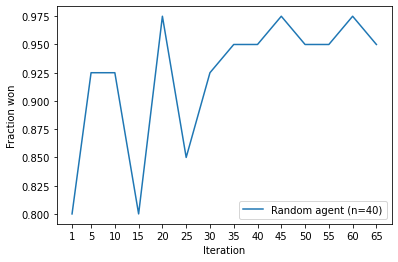
\includegraphics[height=5cm, keepaspectratio]{validation_tictactoe.png}
    }
    \hfill
    \subfloat[Othello $6 \cdot 6$ field]{
        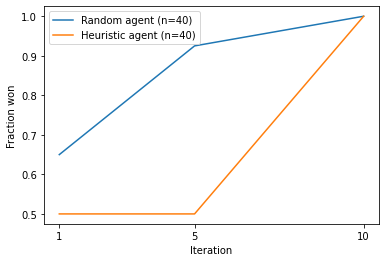
\includegraphics[height=5cm, keepaspectratio]{validation_othello.png}
    }
    \caption{Win-ratio against random baseline in TicTacToe and Othello. Win-ratio is $\frac{\text{gamesWon}}{\text{allGames}}$ }
    \label{tictactoe_performance}
\end{figure}

\section{Application}
\subsection{Naive Run}
\paragraph{Hypothesis} The naive implementation without any Abalone specific modifications converges to optimal play.
\paragraph{Setup} Run pipeline on Balthazar.

\begin{table}[!h]
    \begin{center}
        \begin{tabular}{ c|c }
            Name                       & Value   \\
            \hline
            \hline
            num\_MCTS\_sims            & 60      \\
            num\_self\_play\_workers   & 2       \\
            num\_arena\_workers        & 2       \\
            maxlen\_experience\_buffer & 960,000 \\
        \end{tabular}
    \end{center}
    \caption{The parameters for the naive run on Balthazar}
\end{table}

\paragraph{Result} No improvement in playing performance, cf. figure \ref{performance_local_naive}
\begin{figure}[!h]
    \centering
    \subfloat[The win-ratio]{
        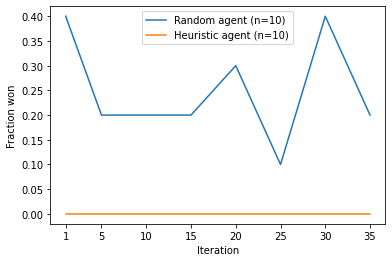
\includegraphics[height=5cm, keepaspectratio]{performance_local_win_ratio.png}
    }
    \hfill
    \subfloat[The cumulative reward]{
        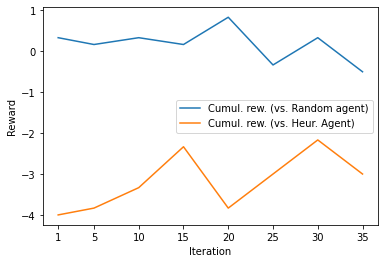
\includegraphics[height=5cm, keepaspectratio]{performance_local_reward.png}
    }
    \caption{The training performance for the naive run}
    \label{performance_local_naive}
\end{figure}

\subsection{Naive Run with large NN}
\paragraph{Hypothesis} The naive implementation without any Abalone specific modifications converges to optimal play with the large NN.
\paragraph{Setup} Run pipeline on Balthazar.

\begin{table}[!h]
    \begin{center}
        \begin{tabular}{ c|c }
            Name                       & Value   \\
            \hline
            \hline
            num\_MCTS\_sims            & 60      \\
            num\_self\_play\_workers   & 2       \\
            num\_arena\_workers        & 2       \\
            maxlen\_experience\_buffer & 960,000 \\
            nnet\_size                 & large   \\
        \end{tabular}
    \end{center}
    \caption{The parameters for the naive run on Balthazar}
\end{table}

\paragraph{Result} No improvement in playing performance, cf. figure \ref{performance_local_naive_large}. The network seems to have a bug leading to strong divergence. We decided to discard the implementation for the time being as the inference and training of the network took approximately 30\% longer.
\begin{figure}[!h]
    \centering
    \subfloat[The win-ratio]{
        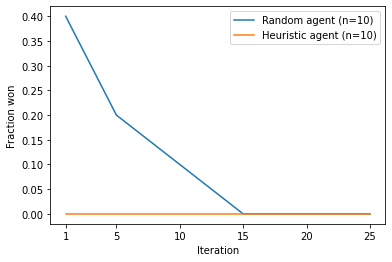
\includegraphics[height=5cm, keepaspectratio]{performance_local_naive_large_win_ratio.png}
    }
    \hfill
    \subfloat[The cumulative reward]{
        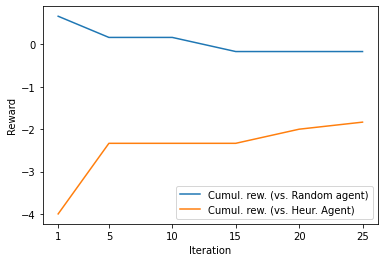
\includegraphics[height=5cm, keepaspectratio]{performance_local_naive_large_cumul_reward.png}
    }
    \caption{The training performance for the naive run with the large NN}
    \label{performance_local_naive_large}
\end{figure}

\subsection{Scaled naive Run}
\paragraph{Hypothesis} The naive implementation without any Abalone specific modifications converges to optimal play on a larger machine with a bigger buffer and more workers.
\paragraph{Setup} Run pipeline on Melchior.
\paragraph{Result} No improvement in playing performance, divergence, cf. figure \ref{performance_remote_naive}
\begin{figure}[!h]
    \centering
    \subfloat[The win-ratio of the naive implementation]{
        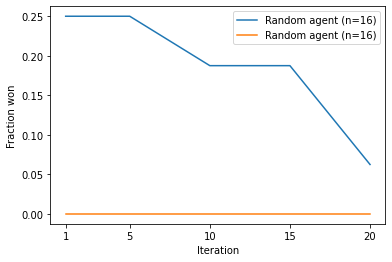
\includegraphics[height=5cm, keepaspectratio]{performance_remote_naive_win_ratio.png}
    }
    \hfill
    \subfloat[The cumulative reward recieved by the naive implementation]{
        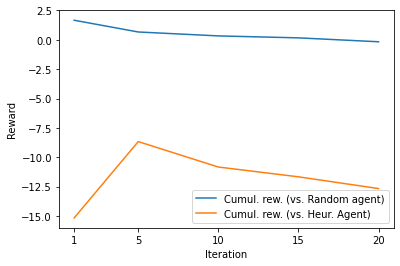
\includegraphics[height=5cm, keepaspectratio]{performance_remote_naive_reward.png}
    }
    \caption{}
    \label{performance_remote_naive}
\end{figure}

\subsection{Reward Distribution}
\paragraph{Hypothesis} The distribution of game results $z$ is uneven.
\paragraph{Setup} Plot histogram of $z$ in experience buffer of previous run.
\paragraph{Result} Most of the games end up as drawn or with minor advantage for one player, cf. figure \ref{distribution_of_rewards}).

\begin{figure}[!h]
    \centering
    \subfloat[The experience buffer after the fifth iteration]{
        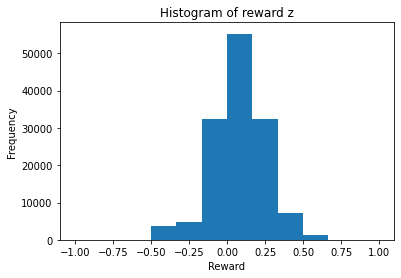
\includegraphics[height=5cm, keepaspectratio]{performance_local_exp_buffer_5.png}
    }
    \hfill
    \subfloat[The experience buffer after the twentieth iteration]{
        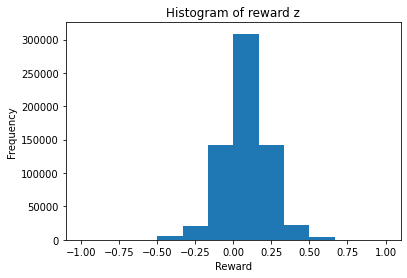
\includegraphics[height=5cm, keepaspectratio]{performance_local_exp_buffer_20.png}
    }
    \caption{Distribution of $z$ in experience buffer of the naive run on Balthazar.}
    \label{distribution_of_rewards}
\end{figure}

\subsection{Scaled warmed-up Run}
\paragraph{Hypothesis} Pretraining the network on experience generated by Verloop's minimax against a random player nudges the network towards more aggressive play. The resulting experience buffer has stronger signals $z$, which improves performance.

\paragraph{Setup} Run pipeline on Melchior with pretrained network.

\begin{table}[!h]
    \begin{center}
        \begin{tabular}{ c|c }
            Name        & Value \\
            \hline
            \hline
            load\_model & true  \\
        \end{tabular}
    \end{center}
    \caption{The parameters for the validation runs}
\end{table}

\paragraph{Result} The experience buffer during different iterations of the training run looks promising. The distribution shows much higher rewards, many games even ending before the cutoff of 200 moves, cf. figure \ref{performance_remote_warmed_up_exp_buffer}.

\begin{figure}[!h]
    \centering
    \subfloat[The win-ratio of the naive implementation]{
        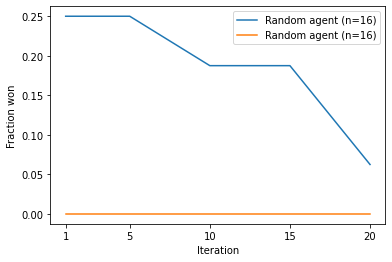
\includegraphics[height=5cm, keepaspectratio]{performance_remote_naive_win_ratio.png}
    }
    \hfill
    \subfloat[The cumulative reward recieved by the naive implementation]{
        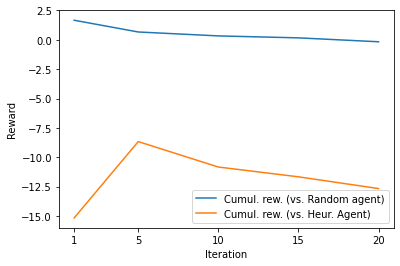
\includegraphics[height=5cm, keepaspectratio]{performance_remote_naive_reward.png}
    }
    \caption{}
    \label{performance_remote_warmed_up}
\end{figure}

\begin{figure}[!h]
    \centering
    \subfloat[The experience buffer after the first iteration]{
        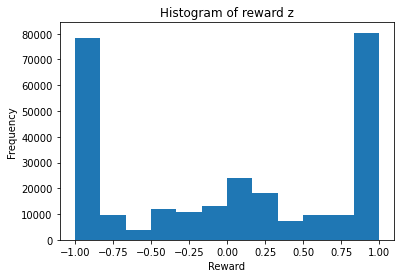
\includegraphics[height=5cm, keepaspectratio]{performance_remote_warmed_up_exp_buffer_1.png}
    }
    \hfill
    \subfloat[The experience buffer after the tenth iteration]{
        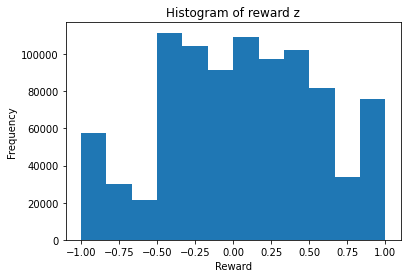
\includegraphics[height=5cm, keepaspectratio]{performance_remote_warmed_up_exp_buffer_10.png}
    }
    \caption{Initially the buffer is still filled with the experience from the prewarming phase, where all games ended with eiter -1 or 1 reward.}
    \label{performance_remote_warmed_up_exp_buffer}
\end{figure}

\begin{figure}[!h]
    \centering
    \subfloat[The agent shows strong play, drawing against the heuristic agent]{
        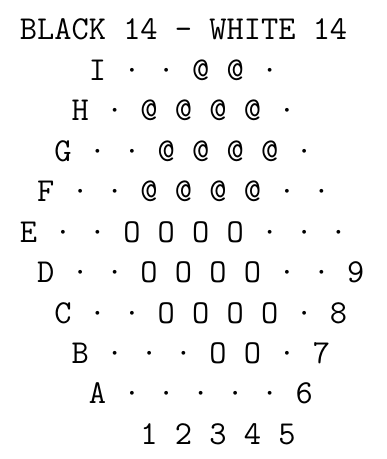
\includegraphics[height=5cm, keepaspectratio]{warmed_up_net_strong_play.png}
    }
    \subfloat[The agent shows weak play, loosing formation and getting pressed against the brink of the board]{
        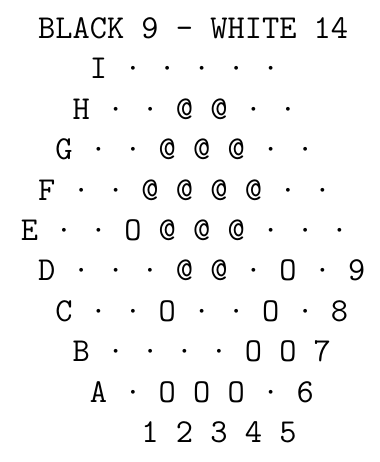
\includegraphics[height=5cm, keepaspectratio]{warmed_up_net_weak_play.png}
    }
    \caption{The final board positions against heuristic player, during training iteration 10 with the warmed up NN}
    \label{performance_remote_warmed_up_heuristic}
\end{figure}

\subsection{Scaled Run with adjusted Reward $z$}
\paragraph{Hypothesis} The reward function provides no penalty for long matches, that result in a draw.
\paragraph{Setup} Run pipeline on Melchior with adjusted reward function. Each turn has a reward of $-0.001$, for a maximum game length of 200 that is a maximum of $-0.2$. The other rewards remain unchanged.

\paragraph{Result} Inconclusive for the amount of iterations performed. A tendency of improvement is present.
\begin{figure}[!h]
    \centering
    \subfloat[The win-ratio of the naive implementation]{
        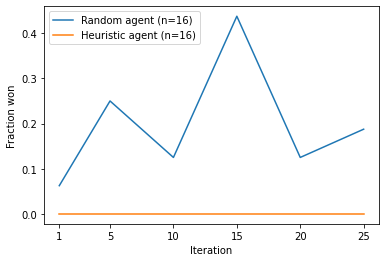
\includegraphics[height=5cm, keepaspectratio]{performance_remote_diff_z_win_ratio.png}
    }
    \hfill
    \subfloat[The cumulative reward recieved by the naive implementation]{
        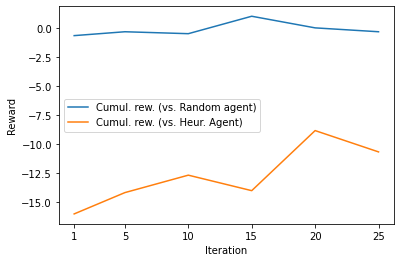
\includegraphics[height=5cm, keepaspectratio]{performance_remote_diff_z_cumul_reward.png}
    }
    \caption{}
    \label{performance_remote_diff_z}
\end{figure}

\subsection{Runtime of Experiments}
\paragraph{Hypothesis} The training of the neural network has become a bottlenet.
\paragraph{Setup} Compare lengths of training iterations on Balthazar and Melchior.

\paragraph{Result} Due to the parallel nature, self-play games are generated continuously. The longer one training iteration takes, the bigger the backlog of new games becomes. One iteration took on average 1h. The training of the network has become the limiting factor, not the generation of self-play games, cf. figure \ref{iteration_duration}. The serialized experience buffer (with Python pickle) with 1,000,000 items takes 10GB of storage. As the entire buffer is used for training, the long training duration is to be expected.

\begin{figure}[!h]
    \centering
    \subfloat[Training run on Balthazar]{
        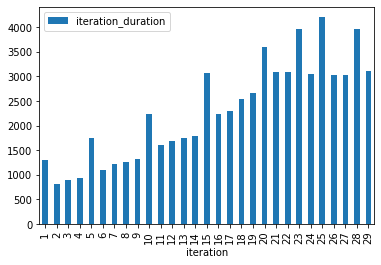
\includegraphics[height=5.2cm, keepaspectratio]{performance_local_iteration_duration.png}
    }
    \hfill
    \subfloat[Training run on Melchior]{
        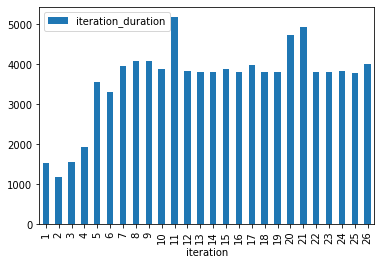
\includegraphics[height=5.2cm, keepaspectratio]{performance_remote_naive_iteration_duration.png}
    }
    \caption{Duration of one training iteration in seconds. The training times stabilize once the experience buffer has reached its maximum size.}
    \label{iteration_duration}
\end{figure}